\documentclass[]{article}
\usepackage{xcolor}
\usepackage{mdframed}
\usepackage{graphicx} 
\usepackage{mcode}
\usepackage{fontawesome}
\usepackage{amsmath}
\usepackage{hyperref} 
\usepackage{xcolor}

% your names and student id's go here: 
\newcommand{\StudentA}{First Student}
\newcommand{\StudentB}{Second Student}
\newcommand{\StudentIdA}{1234567890}
\newcommand{\StudentIdB}{0987654321}

\newcommand{\dueDate}{23.1.2016}

\newcommand \BeginAnswer {\begin{mdframed}[backgroundcolor=blue!15]} 
	\newcommand{\EndAnswer}{\end{mdframed}}
\renewcommand\thesection{Part \Alph{section}-}
\renewcommand\thesubsection{\arabic{subsection}.}
\renewcommand\thesubsubsection{\thesubsection\arabic{subsubsection}}  
\newcommand{\code}{\item[\faKeyboardO]}
\newcommand{\quest}{\item[\faPencil]}

% Title Page
\title{Sparse Representations and Their Applications in Signal and Image Processing \break\\
	Home Work 3: On-line Dictionary Learning for Denoising}

\author{Submitted by: \begin{tabular}{cc}
		\StudentA & \StudentIdA \\ 
		\StudentB  & \StudentIdB 
	\end{tabular}}
	\date{due \dueDate}
	
	\begin{document}
		\maketitle
		\section*{Instructions} 
		
		\begin{itemize}
			\item Work should be done in pairs and submitted via moodle. Students wishing to submit on their own need to get permission to do so in advance. 
			\item Submission should include a pdf-file containing the report and all Matlab files you created for this exercise.
			\item You are encouraged (but not obligated) to use \LaTeX\ for your report, and add your answers to the project \texttt{.tex} file that is included with the exercise files. \emph{You will get a 5 point bonus for doing so. However, the maximal grade will be 100 in any case for the exercise}.
			%	\item The items that require you to code or write an answer have an icon of keyboard or pen respectively.
			%	\BeginAnswer
			%	If you decide to submit your file in LaTeX, make sure your answers and figures are placed inside a 
			%	\texttt{\textbackslash BeginAnswer} \ldots \texttt{\textbackslash EndAnswer} 
			%	block that places what you added in a box such as this one.
			%	\EndAnswer 
			\item Write your own code. This exercise is meant to teach you how the different algorithms operate.
			\item Indent and highlight the Matlab code you attach to the report. In LaTeX this is done using the command: \lstinline|\lstinputlisting{<filename>}| from the package \lstinline|mcode.sty|, which is already included in the homework laTeX file. 
			\item Use sparse type vectors and matrices in your code when it is appropriate.
			\item Questions regarding the exercise should be asked in the course forum in moodle, e-mails about the exercises will not be answered.    
		\end{itemize}
		
		\section{ Problem Description } 
		You will be following the dictionary learning algorithm described in \cite{mairal2009online}. The process you are going to implement is as follows:
		\subsection{Input Image}
		\begin{itemize}
			\item Choose an interesting Image with texture and rich content. 
			\item The size of the selected image should be $256x256$ or larger.
			\item Corrupt the image with noise with AWGN, with variance $\sigma^2$ ($\sigma = 20$). 
			\item The image should be decomposed into an array of fully-overlapping patches of size $b\times b$ ($b=8$). 
			\item Image patches should have \emph{zero-mean}, do this by subtracting the mean from each patch, but save the means for later. 
			\item You can find all these steps implemented in the supplied matlab file.   
			
		\end{itemize}
		\subsection{Initial Dictionaries ($D_0$ in \cite{mairal2009online})}
		Use the following dictionaries as initialization for the training process
		\begin{itemize}
			\item Random Gaussian dictionary of size $64\times 256$ 
			\item Random Gaussian dictionary of size $64\times 400$   
			\item Truncted wavelet of size $64\times 256$ that is supplied in the file \lstinline|D0.mat|, taken from \cite{sulam2016trainlets}. 
		\end{itemize}
		
		\subsection{Online Dictionary Learning}
		\begin{itemize}
			\item Implement the dictionary learning algorithm from \cite{mairal2009online}
			\begin{itemize}
				\item Algorithm 1 is the main algorithm. Drawing $x$ from $p(x)$ as mentioned in the algorithm means simply to choose a patch at random from the set of extracted patches (i.e., this can be done by picking a random integer \lstinline|i| in the range 1 to \lstinline|size(patches,2)| and setting \lstinline|x=patches(:,i)|). 
				\item Algorithm 2 is used by Algorithm 1. In your implementation of this part you only need a single \lstinline|while| as the \lstinline|for| step that is used in the description of Algorithm 2  can be implemented simply by a matrix multiplication. Take care also not to divide by 0 (it may happen in the algorithm that you will need to divide by an entry in the matrix that is equal to zero. In this case divide by something other than zero). The stopping condition for this algorithm should be the Frobenius norm between subsequent values of $D$, i.e., $\|D_{j}-D_{j-1}\|_{F}\leq \epsilon$ for some small enough $\epsilon$.    
			\end{itemize}
			\item Your code should support two modes:
			\begin{enumerate}
				\item Regular version (i.e. $\eta = 1$) as described in algorithm 1 in the paper. 
				\item Mini-batch mode that support values of $\eta$ bigger than $1$ (see Equation (11) in \cite{mairal2009online}) .   
			\end{enumerate}
			\item Sparse coding 
			\begin{itemize}
				\item Use OMP instead of LARS (which is used in Algorithm 1 in \cite{mairal2009online}).  
				\item Your implementation should support two stopping criteria: 
				\begin{enumerate}
					\item If the sparsity reached a certain threshold: \lstinline|max_sparsity|
					\item If the error ($\|r\|^2$) is below a \lstinline|noise_threshold|  
					
				\end{enumerate} 
				\item \emph{Note:} OMP over all the data is also implemented in the supplied \lstinline|RunMe.m|. You may re-use it if you want.   
			\end{itemize}
			\item Use a parameter named \lstinline|train_size| to limit the amount of iterations in the algorithm (denoted by $T$ in \cite{mairal2009online}). 
			
			\item Your function should look like this in order to use the supplied code: 
			\lstinline|Dictionary = odl(patches,D0,train_size,max_sparsity,noise_threshold,eta)|
			
		\end{itemize} 
		
		\section{Implementation \& Running}
		\subsection{Implementation notes}
		\begin{itemize}
			\item Set $\sigma =20$ and $b=8$. 
			\item Set \lstinline|max_sparsity=20|. This quantity might need to be reduced due to numerical issues  depending on the richness of texture of the image you choose.  
			\item Set the \lstinline|noise_threshold| to be $C\sigma^2 b^2$, where $C=1.15$.  
			\item First pick your favorite initial dictionary (the one that gives the best results) when running with $\eta =1$, and then try to see if a different value of $\eta$ can help reconstruction accuracy and convergence speed. Pick one of these values as you see fit. 
			
			\item Every 500 iterations or so of the dictionary learning function compute the \emph{over all} representation error (on all the data) and the average sparsity of the representation. Plot and compare the graphs of the different experiments you  perform.
			\item Take a look at (and put in your report) the dictionary you are getting by plotting the atoms (a 16 by 16 grid of 8 by 8 patches in the case of the truncated wavelets dictionary (and the first Gaussian Dictionary), and a 20 by 20 grid in the case of the second Gaussian dictionary). Your report should include a comparison between how the dictionary looks before and after the training.  
			\item Compare the different initial dictionaries and the running modes (values of $\eta$). Compare the root mean square error (RMSE) of the representation and the PSNR before and after the dictionary learning phase. Discuss your results and try to explain them.  
		\end{itemize}
		
		\subsection{Supplied Code} 
		You are supplied with a \lstinline|RunMe.m| file that splits the image into patches and performs pursuit on the extracted patches to get the representation, thus implementing almost anything you need for this exercise, except for the actual dictionary learning function (commented out in block E). 
		Feel free to use it, but if you do, you are required to explain what it does. To this end the code is partitioned into blocks (that are marked by a capital letter, e.g. \lstinline|%A|). Explain using no more than two lines of comments what each block does.  
		
		These are the results after running ODL on a $350 \times 234$ pixel image: 
		\begin{center}
			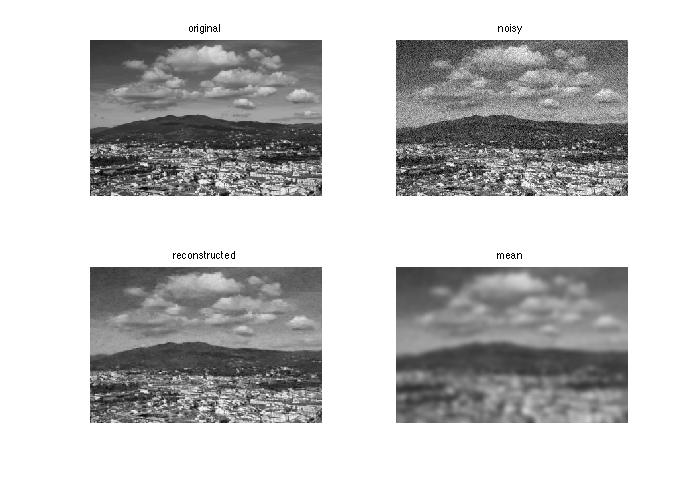
\includegraphics[width=1\linewidth]{fig/data}
			\lstinline|noisy PSNR = 24.4193, reconstructed PSNR = 30.5649|
		\end{center}
		Try to improve upon these.
		
		\section*{Wrap Up}
		\begin{itemize}
			\code Create the file \lstinline|RunMe.m| that can be used to run all the code for this exercise and recreate your results 
			\item Submission in moodle should include two files: 
			\begin{itemize}
				\item Your report in PDF format, named \lstinline|SparseRepHw2_<student #1>_<student #2>.pdf|.
				\item Compressed ZIP file named \lstinline|SparseRepHw2_<student #1>_<student #2>.zip| containing your report and matlab code.  
			\end{itemize}   
		\end{itemize}
		
		\bibliographystyle{plain}
		{\bibliography{hw_refs}}
	\end{document}          
